\chapter{Communication and Utilization of Confidence Values}
	\label{cha:imputation}
	
	Mobile networks are trusted more and more with handling communication that is critical for us: we wait for a call from a loved one to know they arrived safely, we navigate the world without a map using our phones, and we feel assured that if needed, we can call the emergency number at any time.
	But as we trust the mobile network more, so it becomes a potential weak point or a target for an attack, and by extension, we become more vulnerable.
	Thus, mobile networks have to be prepared for internal failure or malicious influence to truly measure up to the trust we give to them.
	
	Just as intelligent people take new information with a pinch of salt, intelligent systems could also process their inputs with a little suspicion.
	Furthermore, when having doubts, people intuitively highlight these doubts when conveying the information further, in a semi-conscious attempt to potentially stop the spread of misinformation.
	Something similar could be important for cognitive network automation, which aims to utilize \ac{DNN}-based cognitive functions for various tasks.
	\acp{DNN} are known to be susceptible to data corruption, which can greatly influence, or even completely break their inference with only slight modifications to the input values \cite{adversarial_examp}.
	The problem is quite similar to people communicating, as cognitive network automation also imagines \acp{CF} conveying processed information between each other.
		
	In this chapter, I discuss a potential solution to the above problem, which mimics human interaction: the communication of confidence values between \acp{CF}.		
	Confidence values are the numerical representation of how reliable each value/observation is in a dataset.
	Figure~\ref{fig:conf_values} illustrates this concept.
	By generating and communicating confidence values between \acp{CF}, the goal is to reduce or even completely eliminate the impact of corrupted data, making the mobile network more robust against failures or malicious attacks.
	
	\begin{figure}[ht]
		\centering
		\includegraphics[width=\linewidth]{figures/12_imputation/conf_values/conf_values.pdf}
		\caption[Illustration of confidence values]{Illustration of confidence values communicated between CFs.}
		\label{fig:conf_values}
	\end{figure}
	
	This chapter details the work published in the following paper:
	
	\begin{publication}
		Robust Deep Learning against Corrupted Data in Cognitive Autonomous Networks \\
		\textit{Márton Kajó, Janik Schnellbach, Stephen S. Mwanje, Georg Carle} \\
		NOMS 2022-2022 IEEE/IFIP Network Operations and Management Symposium, pp. 1-6. IEEE, 2022.
	\end{publication}

	My contributions to the above paper was the partial design, implementation and evaluation of the algorithms, as well as the co-authoring of the paper.
	The discussion in this thesis expands on the paper, by adding further detail to some elements, as well as framing the work in the complete confidence value	discussion.
	The confidence value concept discussed in this chapter is also contained in the following patent application:		
	
	\begin{patent}
		Accounting for Erroneous Data in Learning and Inference of Cognitive Functions through Confidence Indicators \\
		\textit{Anubhab Banerjee, Márton Kajó, Stephen S. Mwanje} \\
		WO, PCT application no.: PCT/EP2021/067609, filed June 2021
	\end{patent}

	The discussion is concluded by some remarks on standardization efforts for \ac{DL} in mobile networks, and how these efforts -- though well meaning -- could slow down the development of new uses cases of \ac{DL}.

	\section{Robust Deep Learning against Corrupted Data in CAN}
		\label{cha:imputation:sec:integrated_imp}

			\subsection{Problem Statement}

				In the \ac{CAN} concept, \acp{CF} implement network automation functionality, likely based on deep neural nets.
				These \acp{CF} either process data which stems directly from the network in the form of measurements, or use preprocessed data from other \acp{CF} as their input.
				Interdependent \acp{CF} create \ac{CF}-chains (Fig.~\ref{fig:cf_chain}), where subsequent \acp{CF} digest the same batch of data in order to realize a complete network automation function.
				An example of this would be an analytics function, which creates insight that is then used by an optimization function to derive actions.
				
				\begin{figure}[ht]
					\centering
					\includegraphics[width=\linewidth]{figures/12_imputation/cf_chain/cf_chain.pdf}
					\caption[Illustration of the propagation of corrupted information in a CF-chain]{Illustration of the propagation of corrupted information in a CF-chain.}
					\label{fig:cf_chain}
				\end{figure}
		
				Any complex system -- such as a network -- is bound to produce erroneous measurements, or even completely fail to report from time to time.
				Mobile networks are prone to generating corrupted data, on account of erroneous measurements (e.g. false \ac{RSRP} reading), the failed delivery of measurements (e.g. packet loss due to congestion), \ac{KPI} computation error (e.g. division by zero), etc.
				Unfortunately, as most \ac{DL} models are based on \acp{DNN}, \ac{CF}-chains might not be robust against such data corruption.
				\acp{DNN} are usually trained on complete datasets, and don't have any indication on how dependable each observation is, apart from how useful it is in generating the required output.
				Because of this, \acp{DNN} often learn to only utilize the few most useful inputs in their models during training, which makes them likely to fail if one or multiple of those values becomes corrupted during inference.
				This situation is further worsened in \ac{CF}-chains, where a single corrupted input can cause a \ac{CF} to produce multiple corrupted outputs, with each step of the chain multiplying the effect (Fig.~\ref{fig:cf_chain}).		
				If critical network management decisions are based on such corrupted data, the \ac{CAN} system could easily misconfigure the network, leading to low service quality or even outage in the worst cases.
				However, if the communicated data includes confidence indicators that highlight the corrupted values, the \acp{CF} can learn to disregard these, and use other features if available, or fall back to some simpler logic.
				The communication of confidence values could hinder or stop the propagation of corrupted data, thus making the network robust against this threat.
		
				This work focuses on the simplest setting in which confidence values can be utilized: the values are either completely correct ($1.0$ confidence), or are completely corrupted ($0.0$ confidence).
				For now, it is of no concern how these confidence values can be generated.
				It is assumed that data corruption is unintended, and the network element that produces corrupted outputs also highlights these by outputting correct confidence values.
				The question is whether it is even possible for \ac{DNN}-based \ac{CF} to utilize confidence values effectively, and restore data using them.
				This is a well known scenario in \ac{ML}, called ``imputation'': the act of restoring known-to-be corrupted or missing values in a dataset.

				\urldef{\footurl}\url{https://github.com/nokia/integratedimputation.git}
				The complete code-base and the dataset used in our evaluation is available on GitHub\footnote{\footurl}.
		
			\subsection{CF-chains in Mobile Networks}
			
				% Slicing
				% * DeepCog: Cognitive Network Management in Sliced 5G Networks with Deep Learning                       <- this
				% * DeepSlice: A Deep Learning Approach towards an Efficient and Reliable Network Slicing in 5G Networks <- this
				% * Offline SLA-Constrained Deep Learning for 5G Networks Reliable and Dynamic End-to-End Slicing
				% * Consideration On Automation of 5G Network Slicing with Machine Learning
				
				% Load balancing
				% * A load balancing scheme based on deep-learning in IoT
				% * Load Balancing for Ultradense Networks: A Deep Reinforcement Learning-Based Approach                 <- this
				% * User Association and Load Balancing for Massive MIMO through Deep Learning                           <- this
				
				% Handover optimization
				% * Deep Learning based Adaptive Handover Optimization for Ultra-Dense 5G Mobile Networks                <- this
				% * Prediction-Based Conditional Handover for 5G mm-Wave Networks: A Deep-Learning Approach
				% * Machine-Learning-Based Predictive Handover (our paper)                                               <- this
				
				% Anubhab's papers
				% * On the implementation of Cognitive Autonomous Networks                                               <- this
				% * Optimal configuration determination in Cognitive Autonomous Networks                                 <- this
				% * Game theoretic Conflict Resolution Mechanism for Cognitive Autonomous Networks
				
				Because of their complex requirements, many automated network management/orchestration functions are being or are likely to be implemented using \ac{DL}.
				\textit{Network slicing} management is one such application area, where the goal is to accurately predict and provision the resource requirements of different services, without over- or under-provisioning.
				\ac{DL} models can accurately predict these requirements by correlating indirect indicators and past patterns in similar services \cite{netw_slicing_1, netw_slicing_2}.
				\textit{Load balancing} is an area where \ac{DL}-based functions excel, because of their capability to estimate close-to-optimal association between users and cells for a large number of users, allowing for real-time inference \cite{load_balancing_1, load_balancing_2}.
				\textit{Handover optimization} is a renewed focus of research, because of the extremely low service interruption times required for \ac{URLLC} use cases.
				Predictive handover optimization can achieve these low interruption times, for which \ac{DL} models can be used \cite{ho_opt_1, ho_opt_2}.			
				While not referred to as \acp{CF} explicitly, these management functions fulfill all the requirements to be called ``cognitive'': having strong modeling capabilities and considering a large volume of varied inputs in their learning and subsequent decision-making.		
				
				Chaining such \ac{DL}-based \acp{CF} is already considered in network automation standards.
				The two most important examples of them are:
				\begin{itemize}
					\item
						The real-time \ac{RIC} in the ORAN\footnote{\url{https://www.o-ran.org/}} specifications is an analytics module, which collects performance measurements from the \ac{RAN} and processes them by \acp{CF} called xApps.
						The processed information is then communicated to local automation and radio resource management \acp{CF} in the \ac{RAN} to drive actions on the cells \cite{ric}.
					
					\item
						The \ac{NWDAF} in the 3GPP\footnote{\url{https://www.3gpp.org/}} specifications is an analytics module, which can provide extracted features and predictions to subsequent \acp{CF} \cite{nwdaf}.
				\end{itemize}
				
				Both the real-time \ac{RIC} and the \ac{NWDAF} are preprocessing/analytics \acp{CF}, which provide digested data to subsequent network management functions.
				Both of these modules are based on \ac{ML} algorithms, more than likely some form of \ac{DNN}, in order to be able to achieve sufficient modeling capability and to be able to process large amounts of data.
				If the subsequent \acp{CF} are also \ac{DL}-based, the above two proposals realize the exact \ac{CF}-chains where data corruption can have severe effects.
				
				Apart from the standards discussions, scientific publications regarding \ac{CF}-chains, and the robustness thereof against corrupted data are scarce.
				Our colleagues works investigate how such \ac{DNN}-based \acp{CF} interact with each other, but these evaluations do not cover scenarios where the inputs or outputs of the \acp{CF} contain corrupted information \cite{anu_can_1, anu_can_2}.
				On one hand, it remains to be seen how well data corruption can be detected if it is not directly signaled by the data source. 
				On the other hand, it is also a question how well \acp{CF} can utilize this information if available, a topic which is the focus of this chapter.
		
			\subsection{State-of-the-Art in DL-based Imputation}

				\acp{DNN} are often hard to categorize, because their topology, the training methods, and other hyper-parameters vary with each application.
				Fortunately, two larger architectures have crystallized along which \ac{DL}-based imputation methods can be grouped: \acp{AE} and \acp{GAN}.
				
				\acp{AE} are mainly used in unsupervised learning, their usual goal being feature extraction.
				During training, \acp{AE} learn to encode the data into a latent representation, as well as to reconstruct (decode) the original datapoints from this internal representation.
				For this, \acp{AE} use $2$ sub-nets with mirrored topologies: the encoder $Q$, and the decoder $Q'$.
				The latent representation is constrained by the topology of the \ac{AE}; traditional \acp{AE} have ``narrow'' layers towards the middle, compressing data by using only a few features for the latent representation.
				This constraint forces the learned features to encompass high-level aspects of the data in order to retain as much information as possible, thus encouraging good generalization.
				The learned latent representation is often suitable for subsequent processing steps, such as classification or clustering.
				In this case, the reconstructed datapoints (and the decoder) are only important for training.
				
				\acp{DAE} represent a special type of \ac{AE} architecture \cite{dae}.
				By adding noise to the training data, \acp{DAE} become more robust against corrupted inputs and learn to represent the data internally in a redundant manner.
				\acp{DAE} are used for their capacity to restore corrupted or missing inputs, thus being a prime tool for imputation.
				\ac{MIDA} implements such a \ac{DAE}, using a net topology which the authors refer to as an overcomplete \ac{AE} \cite{mida}.
				Contrary to traditional \acp{AE}, the \ac{AE} in \ac{MIDA} ``widens'' towards the middle, encoding information with more features than the original data.
				To facilitate training for imputation, \ac{MIDA} is trained with randomly missing values (values replaced by $0$).
				Additionally in \ac{MIDA}, a ``mask'' tensor also accompanies the input, which explicitly signals where the data is missing in the input tensor with $0$s (the rest of the mask contains $1$s). 
				\ac{MIDA} gradually learns to replace the missing datapoints by minimizing a reconstruction loss measured between its imputed output and the original, fully present datapoints (Fig.~\ref{fig:dl_imp}).
				In the \ac{DAE} case, correspondingly, the whole \ac{AE} is used in inference.

				\begin{figure}[ht]
					\centering
					\includegraphics[width=\linewidth]{figures/12_imputation/dl_imp/dl_imp.pdf}
					\caption[The MIDA and GAIN architectures]{The MIDA and GAIN architectures.}
					\label{fig:dl_imp}
				\end{figure}
					
				To contrast with \acp{DAE}, one can also consider \acp{VAE}, another subgroup of \acp{AE}.
				Instead of data corruption on the input side, \acp{VAE} manipulate the latent representation: using an additional regularization term, the latent datapoints are forced to fit a predefined distribution, such as a Gaussian.
				Regularization is often performed using the Kullback-Leibler divergence, which is optimized between the encoded distribution and the predefined Gaussian \cite{vae}. 
				Common imputation frameworks that rely on \acp{VAE} are \ac{VAEAC} \cite{vaeac} and \ac{MIWAE} \cite{miwae}.
				
				Generative adversarial nets are also used for unsupervised learning, most often to synthesize believable, but not real samples (such as pictures of human faces) \cite{gan}.
				\acp{GAN} are comprised of two sub-nets, a generator $G$ and a discriminator $D$.
				In the original \ac{GAN} formulation, $G$ generates samples using random noise as input, while $D$ evaluates these samples randomly mixed with original datapoints and tries to guess which one is real and which one is fake.
				The goal of the generator during training is to learn to synthesize samples that are indistinguishable from real datapoints by the discriminator.
				The interaction of $G$ and $D$ is an adversarial zero-sum game.
				During inference, only the generator is used, while the discriminator is usually discarded after training.
				
				\acp{GAIN} utilize the generative capabilities of \acp{GAN} for data imputation \cite{gain}.
				The generator in \ac{GAIN} is an \ac{AE}, which, similarly to \ac{MIDA}, has the task of imputing missing datapoints with believable values.
				The discriminator has the task of distinguishing imputed datapoints from real, fully present datapoints, thus forcing $G$ to perform imputations that are as realistic as possible and difficult for $D$ to detect.
				While the original \ac{GAIN} proposal implements many tricks besides the mask tensor to make the adversarial training work, in our case we could simplify it to a setup that is basically an extension of \ac{MIDA}.
				Here, the discriminator acts as an additional critic besides the reconstruction loss, to further refine the quality of the imputed points (Fig.~\ref{fig:dl_imp}).
				Another \ac{GAN}-based method is \ac{MisGAN} \cite{misgan}.
				The \ac{MisGAN} setup is substantially more complex than \ac{GAIN} and includes two separate generators that first learn to produce complete data and masks.
				Since \ac{MisGAN} has a major focus on images, while our focus is on application to \ac{CF}-chains, we rather focused on \ac{GAIN} in our research.
			
			\subsection{Integrated Imputation}
				
				The imputation algorithms introduced in the previous section were mostly evaluated in scenarios -- such as image or video reconstruction -- where the imputed data is consumed by the end-user.
				For these tasks, the goal is to achieve imputation which is pleasing to the human eye.
				This can cause problems if the same algorithms are used in network management automation tasks, where the imputed data is likely consumed by another \ac{CF}, because aesthetic qualities do not necessarily translate to restored information content.
				Fine details such as high-frequency patterns, or larger features such as slight shifts in the average of values might not be striking to the human observer, but could be of high importance in \ac{ML} tasks, such as classification.
				
				\begin{figure}[ht]
					\centering
					\includegraphics[width=0.8\linewidth]{figures/12_imputation/integrated_imp/integrated_imp.pdf}
					\caption[Integrated imputation]{Imputation integrated with an ML task, using DNNs.}
					\label{fig:integrated_imp}
				\end{figure}	
				
				\ac{DL}-based imputation methods can learn how to replace missing values based on correlation with present values, or previously encountered patterns in sequential data.
				Often, these rules are not immediately apparent, rather, only visible in latent features, which the imputation method has to extract from the data during training.
				\acp{DNN} are the cutting-edge tools for extracting such latent features, being capable of forming an unprecedented ``understanding'' of the internal behavior of the data they are trained on.
				This is also the reason why \acp{DNN} excel in other \ac{ML} tasks and are likely to be used for many \acp{CF} in network management automation.
				
				If a \ac{DNN}-based imputation module precedes a \ac{DNN}-based \ac{CF}, both neural nets are trained on data from the same source, and likely have to learn the same latent features for their functioning.
				This begs the question whether a standalone imputation module is even necessary.
				Thus, we propose to \textit{integrate the imputation into the \ac{DNN} undertaking the \ac{ML} task} in such scenarios, by preparing it to accept missing-mask tensors accompanying its inputs, as well as feeding it with randomly missing input values during training (Fig.~\ref{fig:integrated_imp}).
				
				Apart from sparing the modeling of the same latent behavior twice -- both during training and inference -- this integration has other beneficial effects:
				\begin{itemize}
					\item 
					The \ac{DNN} can tie the imputation to the actual \ac{ML} task, thereby only learning to ``reconstruct'' the necessary task-relevant features, and disregarding task-irrelevant ones (as opposed to learning to reconstruct all features with equal importance in a standalone imputation module).
					
					\item
					Training with incomplete data has a regularization effect on the model, forcing it to learn generic rules which apply to other datasets from the same source and avoid overtraining.
					This effect is beneficial in cases where the training dataset is of a relatively smaller size, an often encountered problem when applying \ac{ML}.
				\end{itemize}

			\subsection{Evaluation Metrics}
			
				Our goal was to evaluate imputation in two ways: first, quantifying the overall reconstruction precision of the algorithms, and second, assessing the imputations utility as part of a \ac{CF}-chain in the context of network automation.
				As the target \ac{ML} application of this chain, we chose a classification scenario where the task was to assign different mobile network users to previously learned groups based on their individual behavior.
				Similar classification models would be implemented, for example, in network functions undertaking \ac{QoE} estimation for users \cite{qoe_est}, resource estimation for network slicing \cite{netw_slice}, or intrusion detection \cite{intrusion_det}.
				For the evaluation of the classification, a classifier trained on the fully-present dataset is used, which is then fed by the imputed data from the various algorithms during evaluation.
				
				In order to evaluate our proposal of a \ac{CF} with integrated imputation, we also evaluate a classifier, which is trained on missing data accompanied by a corresponding mask, and is directly fed by non-imputed data during evaluation.
				This classifier is referred to as \ac{ICI}.
				
				To compare the algorithms in the above two capacities, the following two metrics are used:
				\begin{itemize}
					\item
						\textbf{\ac{MSE}} reflects the similarity between the original data without missing values ($Y$) and the imputed data ($\hat{Y}$), indicating the overall precision of reconstruction.
%						\begin{equation}
%							MSE = \frac{1}{nd} \sum_{i}^{n} \sum_{j}^{d}  (Y_{ij} - \hat{Y}_{ij})^2,
%						\end{equation}
%						\noindent{}where $d$ refers to the number of values/features in an observation and $n$ the number of observations in the dataset.
						The \ac{MSE} is measured on the output of the imputation methods.
						\ac{MSE} is not a good indicator of information content, because the quadratic nature allows the oversight of small features, instead emphasizing larger errors in the reconstruction, which can lead to the loss of information that is critical for the clustering task.
						Nonetheless, \ac{MSE} is an important and intuitive measure of precision, utilized by most of the \ac{DL}-based imputation methods for training.
					
					\item
						\textbf{\ac{ACC}} indicates the proportion of correctly classified observations against the total number of observations in a dataset:
						\begin{equation}
							ACC = \frac{1}{n} \sum_{i}^{n} (C_i == \hat{C}_i),
						\end{equation}
						\noindent{}where $n$ refers to the number of observations in the dataset, $==$ is the boolean test of equality which produces $1$ if the two values are the same and $0$ otherwise, $C_i$ is the true label of the observations and $\hat{C}_i$ is the predicted label (the output of the classifier).
				\end{itemize}	
			
			\subsection{Simulation Scenario}
			
				\begin{figure}[ht]
					\centering
					\includegraphics[width=0.6\linewidth]{figures/12_imputation/imp_sim_scenario/sim_scenario.pdf}
					\caption[Cell layout in the imputation simulation scenario]{Cell layout in the Helsinki simulation scenario.}
					\label{fig:imp_sim_scenario}
				\end{figure}
			
				In order to be able to evaluate the imputation algorithms for both reconstruction precision, and their utility in an \ac{ML} task, a mobile network simulator was used to generate data.			
				The network simulator allowed us to set up known user classes in the data -- from here on referred to as ``ground truth'' -- against which the classification \ac{ACC} can be measured.
				The simulation scenario was set in the city of Helsinki, where mobile users moved around and used the network to communicate.
				The network is comprised of an outer ring of macro- and an inner circle of microcells, covering a densely populated area of the city harbor (Fig.~\ref{fig:imp_sim_scenario}).
				
				The users were differentiated based on their mobility (stationary, pedestrian, vehicular), and their network usage type (talking using \ac{VoIP}, web-browsing using \ac{HTTP} and transferring files using \ac{FTP}).
				The $8$ user groups -- which constitute the ground truth labels -- were made up of stationary and pedestrian users who used all $3$ traffic types, and vehicular users who used either \ac{VoIP} or \ac{FTP} (Tab.~\ref{tab:imp_user_groups}).
				The simulation contained $400$ users, an even distribution of $50$ users from each of the $8$ user groups.
				The whole dataset was split into $5$ folds for cross-validation: in every fold, $10$ users of each group were selected randomly to make up the validation dataset, while the rest of the users' data was used for training the models.
				Through the $5$ folds, each user was guaranteed to be in the validation group once.
				
				\begin{table}[t]
					\centering
					\renewcommand*{\arraystretch}{1.25}
					\begin{tabular}{l|c|c|c|c}
						& Label            & Traffic   & Speed [km/h] & Occupied area	\\
						\hline
						$0$ & Stationary 1 & \ac{FTP}  & $0$          & Inner \& outer	\\
						$1$ & Stationary 2 & \ac{VoIP} & $0$          & Inner \& outer	\\
						$2$ & Stationary 3 & \ac{HTTP} & $0$          & Inner \& outer	\\
						$3$ & Pedestrian 1 & \ac{FTP}  & $4$ - $10$   & Inner circle	\\
						$4$ & Pedestrian 2 & \ac{VoIP} & $4$ - $10$   & Inner circle	\\
						$5$ & Pedestrian 3 & \ac{HTTP} & $4$ - $10$   & Inner circle	\\
						$6$ & Vehicular 1  & \ac{FTP}  & $10$ - $100$ & Outer ring		\\
						$7$ & Vehicular 2  & \ac{VoIP} & $10$ - $100$ & Outer ring		\\
					\end{tabular}
					\caption{User groups in the simulation scenario.}
					\label{tab:imp_user_groups}
				\end{table}			
				
				% 0: downlink_throughput_bits_s
				% 1: uplink_throughput_bits_s
				% 2: serving_cell_rsrp
				% 3: serving_cell_ul_rsrp
				% 4: num_allocated_PRBs
				% 5: rrc_rlf
				% 6: rrc_selsig
				% 7: rrc_rlfsig
				% 8: rrc_con
				% 9: rrc_idle
				% 10: rrc_hosig
				% 11: setting_id			
				
				The user classification is based on indirect measurements, which can realistically be collected by the mobile network without running into privacy issues.
				The collected data contained:
				\begin{itemize}
					\item
					Throughput in bits/sec for downlink and uplink.
					
					\item
					\ac{RSRP} in dBm for the serving cell for downlink and uplink.
					
					\item
					The number of allocated \acp{PRB} for the user.
					
					\item
					Indicator flags for the different \ac{RRC} states, such as connected, \ac{RLF}, handover signaling, idle etc. ...
				\end{itemize}
				\noindent A total of $11$ values were collected every $5$ seconds for every user.		
				The simulation ran for $2560$ time steps, which corresponds to about $3.5$ hours of simulated time in total.
				For each user, the $2560$-long overall sequence was then split into $256$-long sequences with an overlap of $128$ steps, which resulted in a final training dataset shape of $5760 \times 256 \times 11$, and a validation dataset shape of $1440 \times 256 \times 11$ in each fold.
				The algorithms were trained $5$ times, once for each of the $5$ folds of data.
				The results shown below are averaged across these trainings, to reduce the variance in the metrics.
				
				% (5760, 11, 256)
				% (1440, 11, 256)
			
			\subsection{Evaluated Imputation Methods}
			
				We chose two \ac{DL}-based imputation methods to evaluate in this work, one for each architecture: \ac{MIDA} to represent \ac{AE}-based methods, and \ac{GAIN} to represent \ac{GAN}-based methods.
				Both algorithms can be seen as the purest, natural forms of their respective architectures, where other methods such as \ac{MisGAN} and \ac{MIWAE} are more complex, and in our experience harder to use. 
				Another consideration in this choice was the logical transition between the methods: as previously stated, \ac{GAIN} can also be seen as the \ac{GAN}-style extension of \ac{MIDA}, utilizing an additional discriminator net during training to further tune the imputation (Fig.~\ref{fig:dl_imp}).
				This logic leads to an important aspect of our evaluation: we reuse neural net topologies between methods, in order to remove performance difference stemming from simply more or less powerful nets.
				
				Unlike the more traditional datasets originally used in the evaluation of both algorithms, our dataset has an additional time dimension. 
				Because of this extra dimension, it is generally not advantageous to process our data by a fully-connected net that was used by the authors of other works.
				Therefore, we have adapted the topologies of \ac{MIDA} and \ac{GAIN} to \acp{CNN}, which are more suited to process fixed-length time-series data.
				The \ac{AE} topology is the same between \ac{MIDA} and \ac{GAIN}, both made up of an encoder which uses $1$-dimensional deconvolutional and upsampling layers, and a decoder using $1$-dimensional convolutional and average-pooling layers, with a few batch-normalization layers in-between.
				The \ac{GAIN} discriminator is a smaller, simpler version of the \ac{AE} using less of the same layers, while the classifier net is made up of $1$-dimensional convolutional and max-pooling layers, with a batch-normalization layer after each convolutional layer.			
				All neural nets use leaky \ac{ReLU} nonlinearities.
				
				While our \ac{MIDA} implementation stays true to the original proposal, we had to modify \ac{GAIN} in order to make it work acceptably for our scenario.
				The original work proposes a ``hint'' mechanism, with which the discriminator in \ac{GAIN} can be more precise in its task of identifying imputed values.
				However, in our scenario, the discriminator turned out to be extremely precise as is, overtraining so easily that we had to forgo the hint mechanism altogether.
				Unfortunately, this still didn't solve the overtraining issue completely.
				To try to further combat the overtraining of the discriminator, we also implemented \ac{GAIN} using a Wasserstein discriminator proposed in \acp{WGAN} \cite{wgan}.
				Wasserstein discriminators are immune to overtraining and saturation problems, and provide a smoother gradient than traditional \ac{GAN} discriminators, thereby improving the stability of adversarial learning.
				This setup is referred to as \ac{WGAIN}.
				
				% mean
				% kNN
				% MICE
				% MissForest
				
				Apart from the \ac{DL}-based methods, more ``traditional'', non-\ac{DL}-based imputation methods are also evaluated: mean imputation, \ac{kNN}, \ac{MICE} and MissForest.
				These methods are included to give a frame of reference for our evaluation, and to potentially show the increase in performance that can be expected when using \ac{DL}-based methods.
				Mean imputation is a good baseline upon which all of the algorithms should only improve, where the missing values are replaced by the mean of the present values.
				\ac{kNN} is an instance-based imputation method \cite{knn}.
				\ac{MICE} is an often cited imputation method, which uses repeated linear regression to refine the imputation \cite{mice}.
				The MissForest algorithm is a random-forest-based imputation method, capable of handling non-linear correlations and high-dimensional data \cite{missforest}.
				All of these methods had ready implementations in our language of choice, Python\footnote{\url{https://www.python.org/}}.

			\subsection{Training for Different Missing Rates and Types}
			
				It is logical to assume that the number of missing values in the dataset governs how well the data can be reconstructed, as well as how precisely the classification task can be undertaken.
				To this extent, we define $r_{mis}$ (missing rate), the ratio of the number of missing values compared to the number of all values in the dataset:
				\begin{equation}
					r_{mis} = \frac{1}{nd} \sum_{i}^{n} \sum_{j}^{d} (X_{ij} == \emptyset),
				\end{equation}
				\noindent{}where $d$ refers to the number of values/features in an observation, $n$ to the number of observations in the dataset, $==$ to the boolean test of equality and $\emptyset$ to not present values.
				
				During inference, large missing rates cause worse reconstruction precision and classification accuracy, because more of the data is missing, breaking correlations and patterns upon which these tasks can be based.
				This negative scaling effect is most visible with traditional imputation methods.
				\ac{DL}-based methods, on the other hand, are trained with a dataset that contains missing values at some preset $r_{mis}$, and function best when faced with the same specific missing rate at inference.
				To explore this effect, we have trained the \ac{ICI} with different fixed $r_{mis}$, and evaluated all models on the range of $r_{mis} \in [0, 0.875]$.
				The resulting \acp{ACC} can be seen in Fig.~\ref{fig:acc_clf}.				
				
				\begin{figure}[ht]
					\centering
					\includegraphics[width=0.6\linewidth]{figures/12_imputation/acc_clf/acc_clf.pdf}
					\caption[ACC of the ICI trained for various missing rates]{ACC of the ICI trained for various missing rates.}
					\label{fig:acc_clf}
				\end{figure}
				
				The \ac{ICI} trained with $r_{mis} = 0$ shows a harsh degradation in \ac{ACC} when it encounters even the smallest amount of missing values.
				This is due to it never learning to use alternate features, basing its function only on the most descriptive input features, which, when missing, break the classification.
				The other models trained with $r_{mis} > 0$ are immediately more resistant to missing values; even the model trained with $r_{mis} =  0.25$ can handle missing rates up to $0.5$ reasonably well.
				In fact, the $r_{mis} =  0.25$ model achieves slightly better performance at $r_{mis} =  0$ than the model trained for this specific scenario; as mentioned previously, integrated imputation has a regularization effect which avoids overtraining, making the model learn rules which are better at generalization.	
				
				\acp{ICI} trained for higher missing rates show degraded performance with low missing rates.
				We believe this is a specific problem of \acp{DNN}; the neurons expect a certain average level of activation.
				If the incoming values are significantly above (as is the case of low $r_{mis}$) or below this expected average, the neurons produce weird outputs, at least in the early layers.
				A very similar phenomenon was described with the famous dropout regularizer, where the solution was to scale activations during inference according to the dropout ratio used during training \cite{dropout}.
				We have tried such scaling on the inputs, but it did not substantially improve our results.
				Theoretically, one could train and save multiple imputation models to match the incoming data's missing rate, but we prefer to avoid this, trying to keep storage and memory usage at a reasonable level.
				Instead, we also trained a classifier, where the training observations had a random $r_{mis}$ picked from the range $[0.0, 0.875]$ with a uniform probability.
				This varying $r_{mis}$ model seems to perform close to perfectly on the whole range, thus, the performance of such varying $r_{mis}$ training will be shown only when discussing parametric (\ac{DNN}-based) models.
				
				A further question is the type of missingness: so far we have discussed and shown \textit{completely random} missingness, where individual values are missing from the data.
				However, this type of missingness is rather rare in reality: most often, larger sequences of the data are missing, involving all values (i.e.: a sequence of observations is not reported).
				To evaluate such a scenario, performance results are also shown where starting from random positions, $8$-long sequences of all values are missing (the number of missing sequences governed by the $r_{mis}$).
				This is referred to as \textit{sequential} missingness.
		
			\subsection{Evaluation Results}
			
				Figure~\ref{fig:mse_ran} shows the achieved \ac{MSE} with standalone imputation methods for completely random missingness.
				At low missing rates, traditional methods are quite competitive with \ac{DL}-based parametric methods, but this changes as the $r_{mis}$ is increased, failing to reach even the mean imputation's performance at really high missing rates.
				We believe this is due to overfitting the sparse present data.
				The single exception to this is \ac{kNN}, which, stemming from the averaging in its functioning, converges to the global mean at large missing rates.
				Out of the \ac{DL}-based methods \ac{MIDA} is the best, with relatively low \ac{MSE} even at extreme missing rates, thanks to its training being purely dedicated to minimizing \ac{MSE} in its reconstruction.
				Overall, the \ac{DL}-based methods achieve quite similar \ac{MSE} across the whole $r_{mis}$ range.
				
				\begin{figure}[ht]
					\centering
					\subfloat[MSE]{
						\includegraphics[width=0.6\linewidth]{figures/12_imputation/mse_ran/mse_ran.pdf}
						\label{fig:mse_ran}
					} \\
					\subfloat[ACC]{
						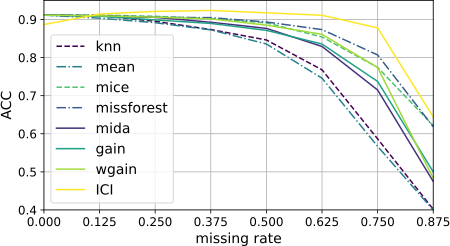
\includegraphics[width=0.6\linewidth]{figures/12_imputation/acc_ran/acc_ran.pdf}
						\label{fig:acc_ran}
					}
					\caption[Imputation performance with completely random missingness]{Imputation performance with completely random missingness.}
				\end{figure}
				
				Figure~\ref{fig:acc_ran} shows the achieved \ac{ACC} on the imputed data for completely random missingness.
				For the classifier, we used the models trained for $r_{mis} = 0$.
				Out of the traditional methods, \ac{MICE} and MissForest are noteworthy, which both surpass the parametric methods at various $r_{mis}$ values, illustrating how low \ac{MSE} does not necessarily translate to restored information.
				Unfortunately, all \ac{DL}-based methods performed quite similarly and worse than MissForest and \ac{MICE} across the whole $r_{mis}$.
				While \ac{WGAIN} did not achieve the best \ac{MSE}, it seems that the Wasserstein discriminator improves the restored information content, achieving the best performance out of the \ac{DL}-based imputation methods.
				
				The \ac{ICI}'s performance also included in the graph with yellow.
				The integrated classifier performs better at every missing rate above $0.0$.
				Furthermore, at moderate to high missing rates, it surpasses the standalone imputation methods by a significant margin.
				At higher missing rates, the imputation methods are likely not able to use correlation in their reconstruction, in which case the classifier is better off disregarding the missing values through the information provided in the mask.
				We will see this effect further emphasized in the sequential missingness case.
		
				Figure~\ref{fig:mse_seq} shows the achieved \ac{MSE} with standalone imputation methods for sequential missingness.
				Correlation-based imputation, which works well in the completely random case -- as seen in Fig.~\ref{fig:mse_ran} -- is seemingly not possible here.
				Both traditional and \ac{DL}-based methods heavily depend on correlation, as none of the methods are capable of achieving a significantly lower \ac{MSE} than mean imputation.
				To impute missing sequences, \ac{DL}-based methods could learn recurring patterns in the data, with which the missing sequences could be imputed.
				However, it seems either such patterns do not exist in our dataset, or the methods were incapable of learning them, as their imputation is only ever marginally better than that of traditional methods, or mean imputation.
				
				\begin{figure}[ht]
					\centering
					\subfloat[MSE]{
						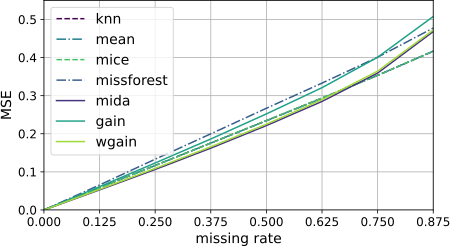
\includegraphics[width=0.6\linewidth]{figures/12_imputation/mse_seq/mse_seq.pdf}
						\label{fig:mse_seq}
					} \\
					\subfloat[ACC]{
						\includegraphics[width=0.6\linewidth]{figures/12_imputation/acc_seq/acc_seq.pdf}
						\label{fig:acc_seq}
					}
					\caption[Imputation performance with sequential missingness]{Imputation performance with sequential missingness.}
				\end{figure}
				
				Figure~\ref{fig:acc_seq} shows the achieved \ac{ACC} on the imputed data for sequential missingness.
				Unfortunately, both traditional and \ac{DL}-based imputation methods' performance barely exceeds the mean imputation's performance.
				It seems that the standalone imputation methods can not restore information in the missing sequences.
				Because the standalone classifier 'pays attention' to the whole sequence, the badly reconstructed values -- which mostly take the value of the average of the sequences -- rather confuse the classifier, instead of helping in the classification process.
				
				Unsurprisingly, the \ac{ICI}'s \ac{ACC} surpasses any standalone imputation method's performance on the whole $r_{mis}$ range.
				Furthermore, the \ac{ACC} only significantly starts to degrade at very high missing rates ($r_{mis} >= 0.75$).
				This is because the classifier trained with missing sequences (and the corresponding mask) learns to only pay attention to parts of the data that are present, in which simple rules can easily identify the right class (type of user in this case).
				
			\subsection{Conclusion and Outlook}
			
				This chapter investigated the utility of confidence values, by focusing on how unintended (non-adversarial) data corruption can be handled in \ac{DL}-based network functions, or chains thereof.
				To this extent, the state-of-the-art in \ac{DL}-based network functions, the standards which define some form of network function chains, and the latest \ac{DL}-based imputation methods were introduced.
				An imputation method was proposed (\ac{ICI}), that is integrated into the network function.
				Standalone methods and \ac{ICI} were evaluated in a mobile network context, with the use of a simulated mobile network dataset and a user classification task.
				
				I would like to highlight that the \ac{ICI} trained with sequential missingness also surpasses the performance of any other classifier on non-missing data (Fig.~\ref{fig:acc_clf}).
				This is caused by the aforementioned regularizing effect of training on missing data; the missing sequences encourage better generalization during training, through which the \ac{ICI} achieves better performance than its peers even in case when there are no missing points in the input.
		
				To summarize, our evaluations show that integrating the imputation into the \ac{DNN} that implements the network function is beneficial in multiple aspects: 
				\begin{itemize}
					\item 
					the network function can show significantly increased performance compared to standalone imputation, retaining its functionality even at large amounts of missing or corrupted data,
					
					\item 
					the processing of missing or corrupted inputs does not require an additional processing step, and
					
					\item
					the network function can show increased performance even with complete inputs.
				\end{itemize}
			
				While our results are promising, one question that came up during our research is how to implement (integrated) imputation into existing architectures.
				This discussion does not only affect imputation, rather, it is part of the larger question on how to incorporate different \ac{DL} tasks into (currently) standardized architectures.
				This topic is covered in the next section.
				
				This work has been preliminary research, as a starting point for the larger topic of confidence value use and communication in \acp{CAN}.
				While the results give me confidence that there is value in the further research of this topic, unfortunately, my time was limited and I could personally not see this topic through.
				Furthermore, it is now clear to me that the topic is larger than what I originally estimated, and could serve as a worthwhile research objective for the next prominent researcher.
				Thus, I don't consider this research topic as concluded, and I hope to be able to continue it in collaboration with others, hopefully someone who is also in pursuit of an academic degree.
				
		\section{On Standardized DL in Mobile Networks}
			\label{cha:imputation:sec:dl_standards}
			
			% https://hackernoon.com/a-brief-history-of-computer-vision-and-convolutional-neural-networks-8fe8aacc79f3
		
			The biggest strength of \acp{DNN} -- as shown in Sec.~\ref{cha:deep_learning:sec:hierarchical_features} -- is their capability to extract abstract representations from low-level features through the construction of hierarchical rules.
			These abstract representations -- communicated between the neural net's layers -- are not preprogrammed, rather, learned during training.
			The importance of learned internal representations is very well illustrated, if we take a look at how image recognition techniques developed over the years.
			While researchers realized quite early that vision is based on hierarchical rules, pre-\ac{DL} methods relied on preprogrammed logical steps and interfaces to detect features at various levels of abstraction.
			One illustrative example of these is the \ac{HOG} algorithm, which finds edges by calculating gradients between pixels in an image \cite{hog}.
			The edges found in \ac{HOG} are compiled into a histogram of directions and magnitudes, which is then matched to other histograms with a \ac{SVM} classifier.
			The individual steps of a \ac{HOG} process can be seen in Fig.~\ref{fig:hog}.

			\begin{figure}[ht]
				\centering
				\includegraphics[width=\linewidth]{figures/12_imputation/hog/hog.pdf}
				\caption[Illustration of HOG processing steps implementing face-detection]{Illustration of HOG processing steps implementing face-detection\footnotemark.}
				\label{fig:hog}
			\end{figure}
			\footnotetext{\url{https://iq.opengenus.org/object-detection-with-histogram-of-oriented-gradients-hog/}}
			
			The step-by-step processing lends itself to an easier understanding, because the data communicated between the steps has a logical, human understandable meaning.
			However, while relatively useful, these step-by-step methods severely underperform \acp{DNN}.
			In the $2012$ \ac{ILSVRC}\footnote{\url{https://image-net.org/challenges/LSVRC/2012/index}} -- the breakthrough introduction of \acp{DNN} to image recognition -- the second best, ``traditional'' Fisher-vector-based image recognition algorithm achieved $26\%$ average error rate, while the first iteration of deep convolutional nets, AlexNet, achieved $16\%$.
			AlexNet did away with individual processing steps, instead realizing a classifier as monolithic \ac{CNN}, which processes raw images and outputs classes in a single step.
			Even today's cutting-edge neural nets cannot improve upon this formula, undertaking complex data processing and control functionality -- such as driving a car -- in a single, end-to-end model (Fig.~\ref{fig:liquid_nn}).
			Imagine, dear Reader, if the \ac{ILSVRC} challenge required entries to work on the precalculated gradients by \ac{HOG}, instead of raw images.
			Would AlexNet have become the landmark it is today, or would another team, in another, less restrictive image recognition challenge, be recognized as the first to introduce \acp{DNN}?
			
			\begin{figure}[ht]
				\centering
				\includegraphics[width=0.8\linewidth]{figures/12_imputation/liquid_nn/liquid_nn.png}
				\caption[Excerpt of a presentation on liquid neural nets driving cars.]{Excerpt of a presentation on liquid neural nets driving cars\footnotemark.}
				\label{fig:liquid_nn}
			\end{figure}
			\footnotetext{\url{https://www.youtube.com/watch?v=IlliqYiRhMU}}
			
			The power of AlexNet came from the freedom to learn descriptive internal representations during training, without human-defined interfaces in the whole end-to-end task.
			Unfortunately, such freedom is hard to realize in mobile networks right now: standards neatly organize functions into compartmentalized modules, each with its own, predefined goal and interface, splitting end-to-end tasks into steps.
			This approach has its historical roots: in older generations, much of the functionality was implemented through dedicated hardware, thus, early mobile networks were indeed made up of individual boxes.
			Unfortunately, this mindset of compartmentalization carried over to the current day, where \ac{DL} tasks are being integrated into the mobile network as separate, human-defined processing steps.
			
			In Fig.~\ref{fig:nwdaf}, an illustration of the standardized \ac{NWDAF} architecture is shown.
			In this framework, the \ac{AnLF} realizes generic \ac{DL} tasks -- such as prediction -- for some predefined use cases.
			Analytics consumers can subscribe to the processed information -- called ``insights'', which either contain processed data or discrete events -- and act on them by changing network parameters using simple, predefined rules.
			While trying to stay flexible, this and similar standards usually fall prey to trying to define in what format data can be communicated between steps, as well as trying to set the purpose of each processing step.
			In my opinion, such a standardized architecture limits the usefulness of \ac{DL} in mobile networks, by hard-coding processes and interfaces, preventing the implementation of new functionality based on \ac{DL} that does not fit the predefined functions.
			This effectively locks \ac{DL} into already standardized functionality.
			
			\begin{figure}[ht]
				\centering
				\includegraphics[width=0.8\linewidth]{figures/12_imputation/nwdaf/nwdaf.pdf}
				\caption[NWDAF architecture]{The NWDAF architecture.}
				\label{fig:nwdaf}
			\end{figure}
			
			To provide an example, we can try to situate integrated imputation into the \ac{NWDAF} framework.
			Integrated imputation could be included into the \ac{AnLF}, a simple solution from an architectural point of view.
			In this case, however, the model training procedure has to be modified to include the randomized dropout.
			Another option is to have an integrated imputation model in the analytics consumer, with the \ac{NWDAF} solely acting as a data-collector/aggregator system.
			However, in this case, the complete training, model management and inference capability of the \ac{NWDAF} is wasted, circumvented by placing this functionality outside of it.
			All-in-all, I am of the opinion that standardizing \ac{DL} processes hinders more than it helps, and I hope future mobile architectures will change to harmoniously integrate \ac{DL} in a less predefined fashion.

